\documentclass[11pt]{amsart}
\usepackage[a4paper,margin=28mm]{geometry}
\usepackage[T1]{fontenc}
\usepackage{lmodern}
\usepackage{amsmath,amssymb,amsthm,mathtools}
\usepackage{booktabs,array,longtable}
\usepackage{microtype}
\usepackage{xcolor}
\usepackage{tikz}
\usepackage{hyperref}
\usepackage[nameinlink,capitalize,noabbrev]{cleveref}
\usepackage{enumitem}
\hypersetup{colorlinks=true,linkcolor=blue!55!black,citecolor=blue!55!black,urlcolor=blue!55!black,pdftitle={The Exact Zarankiewicz Number Z(13,22,3,3)},pdfauthor={Koyar Afrasyab}}

\newtheorem{theorem}{Theorem}[section]
\newtheorem{lemma}[theorem]{Lemma}
\newtheorem{proposition}[theorem]{Proposition}
\newtheorem{corollary}[theorem]{Corollary}
\newtheorem{definition}[theorem]{Definition}
\newtheorem{remark}[theorem]{Remark}
\newcommand{\Z}{\mathrm Z}
\newcommand{\bin}[2]{\binom{#1}{#2}}
\DeclareMathOperator{\rank}{rank}

\title[The exact value of $\Z(13,22,3,3)$]{The Exact Zarankiewicz Number $\Z(13,22,3,3)$}
\author{Koyar Afrasyab}
\thanks{Independent researcher. Email: \texttt{koyar@kinvectum.com}.}
\date{1 August 2026}
\subjclass[2020]{05C35, 05D99, 68R10, 90C05}
\keywords{Zarankiewicz number, extremal bipartite graph, forbidden submatrix, computer-assisted proof, Farkas certificate, block design}

\begin{document}
\begin{abstract}
The Zarankiewicz number $\Z(m,n,s,t)$ is the maximum number of edges in a bipartite graph with parts of orders $m$ and $n$ containing no copy of $K_{s,t}$. Recent construction search established a $137$-edge $K_{3,3}$-free graph on parts of orders $13$ and $22$, while the best published upper bound recorded for this parameter was $140$. We prove that no $138$-edge example exists and hence determine the exact value
\[
  \Z(13,22,3,3)=137.
\]
The upper bound is a finite, certificate-based computer-assisted proof. Triple counting and a supporting-line penalty reduce a hypothetical $138$-edge graph to $83$ column-degree profiles. Exact rational block-polytope certificates exclude $77$ profiles, and one further profile is removed by an elementary marked-row congruence argument. For each of the five remaining profiles, a marked row produces a twelve-point residual packing and a leave multigraph. Point-type equations, modular Gram-rank tests, determinant-square conditions, exhaustive leave enumeration, and exact Farkas certificates eliminate every residual case. The accompanying verifier uses integer and rational arithmetic only; floating-point optimization is used solely to discover certificates and is not part of the proof trust boundary.
\end{abstract}
\maketitle

\section{Introduction}
The Zarankiewicz problem asks for the maximum number of edges in a bipartite graph avoiding a specified complete bipartite subgraph. It was posed by Zarankiewicz in 1951 \cite{Zarankiewicz1951} and was placed in its modern extremal form by K\H{o}v\'ari, S\'os and Tur\'an \cite{KST1954}. Although the asymptotic theory is extensive, exact values for moderate finite parameters remain difficult. The difficulty is particularly pronounced for $K_{3,3}$-free graphs: useful counting inequalities leave a small but highly structured set of integer configurations, while direct exhaustive search suffers from severe symmetry and proof-certification costs.

Write $\Z(m,n,s,t)$ for the maximum number of edges in a subgraph of $K_{m,n}$ containing no $K_{s,t}$. Roman's linear-programming framework \cite{Roman1975} and later strengthened relaxations \cite{DaviesGillHorsley2026} provide effective finite upper bounds. SAT-based methods have also been developed for exact finite cases \cite{Tan2022}. On the lower-bound side, Bhan, Nobili and Langer \cite{BhanNobiliLanger2026} recently obtained a $137$-edge construction for the present parameter, while the prior upper bound was $140$ \cite{DaviesGillHorsley2026}. Thus
\[
  137\le \Z(13,22,3,3)\le140.
\]
Their work also determined three neighboring exact values, including $\Z(12,22,3,3)=132$.

The contribution of this paper is the matching upper bound.

\begin{theorem}\label{thm:main}
There is no $13\times22$ binary matrix with $138$ ones and no all-one $3\times3$ submatrix. Consequently,
\[
  \boxed{\Z(13,22,3,3)=137}.
\]
\end{theorem}

The proof is computer-assisted but certificate based. It is not a report of a mixed-integer solver returning ``infeasible.'' Every load-bearing numerical assertion is replayed by short exact-arithmetic programs from explicit finite data. The architecture has three layers.

\begin{enumerate}[label=(\roman*)]
\item A global degree-profile argument reduces $138$ edges to $83$ profiles and eliminates $77$ by exact rational Farkas certificates.
\item A direct marked-row congruence argument excludes the exceptional profile $6^{18}7^3 9^1$.
\item The remaining five profiles are reduced to finite residual block-design problems on twelve points. Exhaustive leave-multigraph enumeration, necessary Gram conditions, and exact Farkas certificates exclude all residual cases.
\end{enumerate}

The accompanying repository includes an explicit $137$-edge witness, all certificates, the exhaustive enumerator, independent profile enumerators, and a one-command verification gate, so the computation can be independently reproduced.

\section{Block formulation and the lower bound}
Let $X=[13]$. Identify the $j$th column of a binary $13\times22$ matrix with its support $E_j\subseteq X$, and put $d_j=|E_j|$. For each triple $T\in\binom{X}{3}$, define
\[
  \lambda_T=|\{j:T\subseteq E_j\}|.
\]
The matrix is $K_{3,3}$-free if and only if
\begin{equation}\label{eq:triple-capacity}
  \lambda_T\le2 \qquad(T\in\binom{X}{3}).
\end{equation}
Repeated columns are allowed throughout.

The supplementary file \texttt{proof/data/z13\_22\_137\_blocks.json} contains $22$ blocks with total size $137$. Direct enumeration of all $\binom{13}{3}=286$ triples verifies \eqref{eq:triple-capacity}. Thus
\begin{equation}\label{eq:lower}
  \Z(13,22,3,3)\ge137.
\end{equation}
The same lower bound was first reported in \cite{BhanNobiliLanger2026}. A matrix plot of the independently checked witness is shown in \cref{fig:witness}; its block supports are listed in \cref{app:witness}.

\begin{figure}[ht]
\centering
\resizebox{0.92\textwidth}{!}{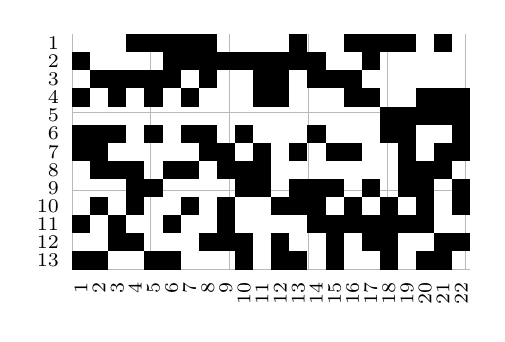
\begin{tikzpicture}[x=0.23cm,y=0.23cm]
  \draw[gray!55,very thin] (0,0) grid (22,13);
  \fill (0,11) rectangle ++(1,1);
  \fill (0,9) rectangle ++(1,1);
  \fill (0,7) rectangle ++(1,1);
  \fill (0,6) rectangle ++(1,1);
  \fill (0,2) rectangle ++(1,1);
  \fill (0,0) rectangle ++(1,1);
  \fill (1,10) rectangle ++(1,1);
  \fill (1,7) rectangle ++(1,1);
  \fill (1,6) rectangle ++(1,1);
  \fill (1,5) rectangle ++(1,1);
  \fill (1,3) rectangle ++(1,1);
  \fill (1,0) rectangle ++(1,1);
  \fill (2,10) rectangle ++(1,1);
  \fill (2,9) rectangle ++(1,1);
  \fill (2,7) rectangle ++(1,1);
  \fill (2,5) rectangle ++(1,1);
  \fill (2,2) rectangle ++(1,1);
  \fill (2,1) rectangle ++(1,1);
  \fill (3,12) rectangle ++(1,1);
  \fill (3,10) rectangle ++(1,1);
  \fill (3,5) rectangle ++(1,1);
  \fill (3,4) rectangle ++(1,1);
  \fill (3,3) rectangle ++(1,1);
  \fill (3,1) rectangle ++(1,1);
  \fill (4,12) rectangle ++(1,1);
  \fill (4,10) rectangle ++(1,1);
  \fill (4,9) rectangle ++(1,1);
  \fill (4,7) rectangle ++(1,1);
  \fill (4,4) rectangle ++(1,1);
  \fill (4,0) rectangle ++(1,1);
  \fill (5,12) rectangle ++(1,1);
  \fill (5,11) rectangle ++(1,1);
  \fill (5,10) rectangle ++(1,1);
  \fill (5,5) rectangle ++(1,1);
  \fill (5,2) rectangle ++(1,1);
  \fill (5,0) rectangle ++(1,1);
  \fill (6,12) rectangle ++(1,1);
  \fill (6,11) rectangle ++(1,1);
  \fill (6,9) rectangle ++(1,1);
  \fill (6,7) rectangle ++(1,1);
  \fill (6,5) rectangle ++(1,1);
  \fill (6,3) rectangle ++(1,1);
  \fill (7,12) rectangle ++(1,1);
  \fill (7,11) rectangle ++(1,1);
  \fill (7,10) rectangle ++(1,1);
  \fill (7,7) rectangle ++(1,1);
  \fill (7,6) rectangle ++(1,1);
  \fill (7,1) rectangle ++(1,1);
  \fill (8,11) rectangle ++(1,1);
  \fill (8,6) rectangle ++(1,1);
  \fill (8,5) rectangle ++(1,1);
  \fill (8,3) rectangle ++(1,1);
  \fill (8,2) rectangle ++(1,1);
  \fill (8,1) rectangle ++(1,1);
  \fill (9,11) rectangle ++(1,1);
  \fill (9,7) rectangle ++(1,1);
  \fill (9,5) rectangle ++(1,1);
  \fill (9,4) rectangle ++(1,1);
  \fill (9,1) rectangle ++(1,1);
  \fill (9,0) rectangle ++(1,1);
  \fill (10,11) rectangle ++(1,1);
  \fill (10,10) rectangle ++(1,1);
  \fill (10,9) rectangle ++(1,1);
  \fill (10,6) rectangle ++(1,1);
  \fill (10,5) rectangle ++(1,1);
  \fill (10,4) rectangle ++(1,1);
  \fill (11,11) rectangle ++(1,1);
  \fill (11,10) rectangle ++(1,1);
  \fill (11,9) rectangle ++(1,1);
  \fill (11,3) rectangle ++(1,1);
  \fill (11,1) rectangle ++(1,1);
  \fill (11,0) rectangle ++(1,1);
  \fill (12,12) rectangle ++(1,1);
  \fill (12,11) rectangle ++(1,1);
  \fill (12,6) rectangle ++(1,1);
  \fill (12,4) rectangle ++(1,1);
  \fill (12,3) rectangle ++(1,1);
  \fill (12,0) rectangle ++(1,1);
  \fill (13,11) rectangle ++(1,1);
  \fill (13,10) rectangle ++(1,1);
  \fill (13,7) rectangle ++(1,1);
  \fill (13,4) rectangle ++(1,1);
  \fill (13,3) rectangle ++(1,1);
  \fill (13,2) rectangle ++(1,1);
  \fill (14,10) rectangle ++(1,1);
  \fill (14,6) rectangle ++(1,1);
  \fill (14,4) rectangle ++(1,1);
  \fill (14,2) rectangle ++(1,1);
  \fill (14,1) rectangle ++(1,1);
  \fill (14,0) rectangle ++(1,1);
  \fill (15,12) rectangle ++(1,1);
  \fill (15,10) rectangle ++(1,1);
  \fill (15,9) rectangle ++(1,1);
  \fill (15,6) rectangle ++(1,1);
  \fill (15,3) rectangle ++(1,1);
  \fill (15,2) rectangle ++(1,1);
  \fill (16,12) rectangle ++(1,1);
  \fill (16,11) rectangle ++(1,1);
  \fill (16,9) rectangle ++(1,1);
  \fill (16,4) rectangle ++(1,1);
  \fill (16,2) rectangle ++(1,1);
  \fill (16,1) rectangle ++(1,1);
  \fill (17,12) rectangle ++(1,1);
  \fill (17,8) rectangle ++(1,1);
  \fill (17,7) rectangle ++(1,1);
  \fill (17,3) rectangle ++(1,1);
  \fill (17,2) rectangle ++(1,1);
  \fill (17,1) rectangle ++(1,1);
  \fill (17,0) rectangle ++(1,1);
  \fill (18,12) rectangle ++(1,1);
  \fill (18,8) rectangle ++(1,1);
  \fill (18,7) rectangle ++(1,1);
  \fill (18,6) rectangle ++(1,1);
  \fill (18,5) rectangle ++(1,1);
  \fill (18,4) rectangle ++(1,1);
  \fill (18,2) rectangle ++(1,1);
  \fill (19,9) rectangle ++(1,1);
  \fill (19,8) rectangle ++(1,1);
  \fill (19,5) rectangle ++(1,1);
  \fill (19,4) rectangle ++(1,1);
  \fill (19,3) rectangle ++(1,1);
  \fill (19,2) rectangle ++(1,1);
  \fill (19,0) rectangle ++(1,1);
  \fill (20,12) rectangle ++(1,1);
  \fill (20,9) rectangle ++(1,1);
  \fill (20,8) rectangle ++(1,1);
  \fill (20,6) rectangle ++(1,1);
  \fill (20,5) rectangle ++(1,1);
  \fill (20,1) rectangle ++(1,1);
  \fill (20,0) rectangle ++(1,1);
  \fill (21,9) rectangle ++(1,1);
  \fill (21,8) rectangle ++(1,1);
  \fill (21,7) rectangle ++(1,1);
  \fill (21,6) rectangle ++(1,1);
  \fill (21,4) rectangle ++(1,1);
  \fill (21,3) rectangle ++(1,1);
  \fill (21,1) rectangle ++(1,1);
  \node[font=\scriptsize,rotate=90,anchor=east] at (0.5,-0.2) {1};
  \node[font=\scriptsize,rotate=90,anchor=east] at (1.5,-0.2) {2};
  \node[font=\scriptsize,rotate=90,anchor=east] at (2.5,-0.2) {3};
  \node[font=\scriptsize,rotate=90,anchor=east] at (3.5,-0.2) {4};
  \node[font=\scriptsize,rotate=90,anchor=east] at (4.5,-0.2) {5};
  \node[font=\scriptsize,rotate=90,anchor=east] at (5.5,-0.2) {6};
  \node[font=\scriptsize,rotate=90,anchor=east] at (6.5,-0.2) {7};
  \node[font=\scriptsize,rotate=90,anchor=east] at (7.5,-0.2) {8};
  \node[font=\scriptsize,rotate=90,anchor=east] at (8.5,-0.2) {9};
  \node[font=\scriptsize,rotate=90,anchor=east] at (9.5,-0.2) {10};
  \node[font=\scriptsize,rotate=90,anchor=east] at (10.5,-0.2) {11};
  \node[font=\scriptsize,rotate=90,anchor=east] at (11.5,-0.2) {12};
  \node[font=\scriptsize,rotate=90,anchor=east] at (12.5,-0.2) {13};
  \node[font=\scriptsize,rotate=90,anchor=east] at (13.5,-0.2) {14};
  \node[font=\scriptsize,rotate=90,anchor=east] at (14.5,-0.2) {15};
  \node[font=\scriptsize,rotate=90,anchor=east] at (15.5,-0.2) {16};
  \node[font=\scriptsize,rotate=90,anchor=east] at (16.5,-0.2) {17};
  \node[font=\scriptsize,rotate=90,anchor=east] at (17.5,-0.2) {18};
  \node[font=\scriptsize,rotate=90,anchor=east] at (18.5,-0.2) {19};
  \node[font=\scriptsize,rotate=90,anchor=east] at (19.5,-0.2) {20};
  \node[font=\scriptsize,rotate=90,anchor=east] at (20.5,-0.2) {21};
  \node[font=\scriptsize,rotate=90,anchor=east] at (21.5,-0.2) {22};
  \node[font=\scriptsize,anchor=east] at (-0.18,12.5) {1};
  \node[font=\scriptsize,anchor=east] at (-0.18,11.5) {2};
  \node[font=\scriptsize,anchor=east] at (-0.18,10.5) {3};
  \node[font=\scriptsize,anchor=east] at (-0.18,9.5) {4};
  \node[font=\scriptsize,anchor=east] at (-0.18,8.5) {5};
  \node[font=\scriptsize,anchor=east] at (-0.18,7.5) {6};
  \node[font=\scriptsize,anchor=east] at (-0.18,6.5) {7};
  \node[font=\scriptsize,anchor=east] at (-0.18,5.5) {8};
  \node[font=\scriptsize,anchor=east] at (-0.18,4.5) {9};
  \node[font=\scriptsize,anchor=east] at (-0.18,3.5) {10};
  \node[font=\scriptsize,anchor=east] at (-0.18,2.5) {11};
  \node[font=\scriptsize,anchor=east] at (-0.18,1.5) {12};
  \node[font=\scriptsize,anchor=east] at (-0.18,0.5) {13};
\end{tikzpicture}}
\caption{A checked $13\times22$ matrix with $137$ ones. Black cells are ones. Every triple of rows is contained in at most two columns.}
\label{fig:witness}
\end{figure}

\section{Global reduction at 138 edges}
Assume for contradiction that blocks $E_1,\dots,E_{22}$ satisfy \eqref{eq:triple-capacity} and
\begin{equation}\label{eq:sumdegree}
  \sum_{j=1}^{22}d_j=138.
\end{equation}
Double counting incidences between blocks and row triples gives
\begin{equation}\label{eq:triplecount}
  \sum_{j=1}^{22}\binom{d_j}{3}
  =\sum_{T\in\binom X3}\lambda_T
  \le2\binom{13}{3}=572.
\end{equation}

Define the integer penalty
\begin{equation}\label{eq:penalty}
  p(d)=\binom d3-15d+70,\qquad 0\le d\le13.
\end{equation}
Its values are
\[
\begin{array}{c|rrrrrrrrrrrrrr}
d&0&1&2&3&4&5&6&7&8&9&10&11&12&13\\\hline
p(d)&70&55&40&26&14&5&0&0&6&19&40&70&110&161.
\end{array}
\]
Thus $p(d)\ge0$, with equality precisely for $d=6,7$. Combining \eqref{eq:sumdegree}--\eqref{eq:penalty},
\begin{equation}\label{eq:penaltybudget}
  \sum_{j=1}^{22}p(d_j)
  =\sum_j\binom{d_j}{3}-15\cdot138+70\cdot22
  \le42.
\end{equation}
Exact integer enumeration of all histograms $(n_0,\dots,n_{13})$ satisfying
\[
  \sum_dn_d=22,
  \qquad \sum_ddn_d=138,
  \qquad \sum_dp(d)n_d\le42
\]
leaves exactly $83$ degree profiles. This is independently regenerated by \texttt{enumerate138.py} and \texttt{verify\_138\_reduction.py}; no degree window is assumed.

\subsection{The block-polytope relaxation}
For a profile $(n_d)$, choose a degree $f$ with $n_f>0$ and, by row symmetry, fix one $f$-block as $F=\{1,\dots,f\}$. For every remaining allowed support $B\subseteq X$, let $x_B\ge0$ denote its multiplicity. Every actual matrix yields an integral feasible point of the following relaxation:
\begin{align}
 \sum_{B\supseteq T}x_B
 &\le2-\mathbf1[T\subseteq F]
 &&(T\in\binom X3), \label{eq:lp-triple}\\
 \sum_{B\ni r}\binom{|B|-1}{2}x_B
 &\le132-\mathbf1[r\in F]\binom{f-1}{2}
 &&(r\in X), \label{eq:lp-row}\\
 \sum_{B\supseteq P}(|B|-2)x_B
 &\le22-\mathbf1[P\subseteq F](f-2)
 &&(P\in\binom X2), \label{eq:lp-pair}\\
 \sum_{|B|=d}x_B
 &=n_d-\mathbf1[d=f]
 &&(d\text{ active}). \label{eq:lp-count}
\end{align}
The row and pair inequalities are nonnegative sums of triple-capacity inequalities; they are retained because they yield much shorter dual certificates.

\begin{lemma}[Exact Farkas criterion]\label{lem:farkas}
Write \eqref{eq:lp-triple}--\eqref{eq:lp-pair} as $Ax\le b$, and \eqref{eq:lp-count} as $Ex=e$, with $x\ge0$. If rational vectors $\alpha\ge0$ and unrestricted $\beta$ satisfy
\[
 A^T\alpha+E^T\beta\ge0,
 \qquad b^T\alpha+e^T\beta<0,
\]
then the profile is impossible.
\end{lemma}
\begin{proof}
For a feasible $x$,
\[
0\le x^T(A^T\alpha+E^T\beta)
=\alpha^TAx+\beta^TEx
\le\alpha^Tb+\beta^Te<0,
\]
a contradiction. This is the standard alternative theorem of Farkas \cite{Farkas1902}.
\end{proof}

The verifier regenerates every subset $B$ of each active degree and checks every dual coefficient using \texttt{fractions.Fraction}. Stored rational certificates exclude $77$ of the $83$ profiles. The six not separated by this global relaxation are
\begin{equation}\label{eq:sixprofiles}
\begin{split}
&6^{18}7^3 9^1,\qquad 6^{16}7^6,\qquad 5^1 6^{14}7^7,\qquad\
5^2 6^{12}7^8,\qquad 4^1 6^{13}7^8,\qquad 5^3 6^{10}7^9.
\end{split}
\end{equation}

\section{Marked-row deficits}
For every triple $T$, put
\[
  \delta_T=2-\lambda_T\ge0,
  \qquad
  D_r=\sum_{T\ni r}\delta_T.
\]
If
\[
 s=572-\sum_j\binom{d_j}{3}
\]
is the unused triple capacity, then
\begin{equation}\label{eq:deficitsum}
  \sum_{r\in X}D_r=3s.
\end{equation}
Since a fixed row belongs to $\binom{12}{2}=66$ triples, each of capacity two,
\begin{equation}\label{eq:deficitformula}
  D_r=132-\sum_{j:r\in E_j}\binom{d_j-1}{2}.
\end{equation}
This formula gives both congruence restrictions and a local design interpretation.

\subsection{The profile $6^{18}7^3 9^1$}
For this profile, $s=23$, so $\sum_rD_r=69$. Contributions from degree-six and degree-seven blocks in \eqref{eq:deficitformula} are $10$ and $15$, both zero modulo five; the degree-nine contribution is $28\equiv3\pmod5$. Thus
\[
 D_r\equiv
 \begin{cases}
 2\pmod5,&r\notin E_9,\\
 4\pmod5,&r\in E_9.
 \end{cases}
\]
The residue-minimal total is $4\cdot2+9\cdot4=44$. Since the actual total is $69$, only five increments of size five are available, and at least eight rows have residue-minimal deficit.

For a row outside the degree-nine block with $D_r=2$, if $a,b$ count degree-six and degree-seven blocks through $r$, then \eqref{eq:deficitformula} gives $2a+3b=26$, hence $(a,b)=(13,0)$ or $(10,2)$. Deleting $r$ leaves blocks of sizes five and six on twelve points. Pair-capacity degrees imply, respectively, total size-five incidence at most $60<65$, or at most $48<50$. Both are impossible. Therefore all four rows outside $E_9$ consume an increment.

At least eight rows inside $E_9$ consequently have $D_r=4$. For such a row, $2a+3b=20$. The case $(a,b)=(10,0)$ is ruled out by the residual degree-nine block: its eight points permit at most three size-five incidences and the other four at most five, totaling $44<50$. Hence each of these at least eight rows lies in exactly two of the three degree-seven columns. Yet any fixed pair of degree-seven columns can share at most two such rows inside $E_9$, since three shared rows together with $E_9$ would form a $K_{3,3}$. The three pairs account for at most six rows, a contradiction.

\begin{proposition}\label{prop:nine}
The profile $6^{18}7^3 9^1$ is impossible.
\end{proposition}

\section{The marked-row leave method}
It remains to exclude the five profiles in \eqref{eq:sixprofiles} containing only degrees four through seven. Fix a row $r$ and delete it from every block containing it. The resulting residual blocks lie on the twelve-point set $X\setminus\{r\}$.

\begin{definition}
The \emph{leave multigraph} $L_r$ has vertex set $X\setminus\{r\}$ and gives the pair $\{x,y\}$ multiplicity $\delta_{rxy}$. Its total edge multiplicity is $D_r$ and every edge multiplicity lies in $\{0,1,2\}$.
\end{definition}

Suppose the residual blocks have active sizes $s$ and that point $x$ occurs in $u_{x,s}$ blocks of size $s$. Pair capacity through $\{r,x\}$ gives
\begin{equation}\label{eq:leave-degree}
 e_x=22-\sum_s(s-1)u_{x,s},
\end{equation}
where $e_x$ is the degree of $x$ in $L_r$. In addition,
\begin{equation}\label{eq:type-totals}
 \sum_xu_{x,s}=s n_s,
 \qquad
 \sum_xe_x=2D_r.
\end{equation}
Equations \eqref{eq:leave-degree}--\eqref{eq:type-totals} give a finite list of point-type multisets.

Let $M$ be the point-by-residual-block incidence matrix. Its Gram matrix $Q=MM^T$ is determined by the point types and the leave:
\begin{equation}\label{eq:gram}
 Q_{xx}=\sum_su_{x,s},
 \qquad
 Q_{xy}=2-\delta_{rxy}\quad(x\ne y).
\end{equation}
Consequently,
\begin{equation}\label{eq:rankcondition}
  \rank_{\mathbb F_p}(Q)\le q
\end{equation}
for every prime $p$, where $q$ is the number of residual blocks. When $q=12$, $M$ is square and
\begin{equation}\label{eq:detsquare}
  \det(Q)=\det(M)^2
\end{equation}
must be a nonnegative integer square. The verifier uses \eqref{eq:rankcondition} for $p=101,103,107$ and \eqref{eq:detsquare} only as necessary conditions. Cases passing these screens are retained.

For every surviving typed leave, the possible residual blocks form a finite linear factorization system. It requires the prescribed incidence count of every point in every size class, the prescribed pair multiplicities $2-\delta_{rxy}$, and the prescribed number of blocks of each size. An integral residual design would give a nonnegative integral solution. Each screened case is instead excluded by an integer-scaled rational Farkas vector whose inequalities are checked over every eligible residual block.

\begin{proposition}[Certified local screen]\label{prop:localscreen}
For each local parameter tuple invoked below, the program \texttt{local\_screen\_general.cpp} enumerates every point-type distribution satisfying \eqref{eq:leave-degree}--\eqref{eq:type-totals}, every loopless leave multigraph with edge multiplicities at most two and the prescribed degree sequence, and every case surviving \eqref{eq:rankcondition} or \eqref{eq:detsquare}. The Python verifier then checks an exact Farkas certificate for every retained factorization case.
\end{proposition}

The proposition is a finite computational statement. Its implementation is deliberately small: the C++ source is approximately four kilobytes, and the certificate checker uses only the Python standard library. The complete enumeration counts used below are summarized in \cref{tab:localcounts}.

\begin{table}[ht]
\centering
\small
\begin{tabular}{@{}llrrr@{}}
\toprule
Branch & Local parameters & type multisets & leaves & certified survivors\\
\midrule
Common $D=7$ & $(a,b)=(5,5)$ & 19 & 8,641 & 0\\
Common $D=7$ & $(a,b)=(8,3)$ & 37 & 6,733 & 4\\
$5^1 6^{14}7^7$, inside & $(a,b)=(6,4)$ & 508 & 43,715 & 0\\
$5^1 6^{14}7^7$, inside & $(a,b)=(3,6)$ & 6 & 534 & 0\\
$5^2 6^{12}7^8$, $c=2$ & $(10,1),(7,3),(4,5)$ & -- & -- & 195+217+28\\
$5^3 6^{10}7^9$, $c=3$ & $(8,2),(5,4),(2,6)$ & -- & -- & 4,746+656+3\\
$4^1 6^{13}7^8$, inside & $(8,3),(5,5)$ & 41+48 & 367+275 & 12+3\\
\bottomrule
\end{tabular}
\caption{Selected exact local-enumeration counts. A dash indicates that only the final screened-case count is used in the proof report.}
\label{tab:localcounts}
\end{table}

\section{The common deficit-seven branch}
Four of the remaining profiles may force a row outside all degree-five blocks with $D_r=7$. If $a,b$ denote the numbers of degree-six and degree-seven columns through $r$, then \eqref{eq:deficitformula} leaves
\[
 (a,b)=(5,5),(8,3),(11,1).
\]
The $(11,1)$ branch has no point-type distribution. For $(5,5)$, all $8{,}641$ leave graphs fail the Gram-rank condition. The $(8,3)$ branch has $37$ point-type distributions and $6{,}733$ leave graphs; four cases survive the Gram screen. Three have immediate exact local Farkas certificates.

The fourth case is fractionally feasible and therefore requires an integral refinement. The verifier enumerates all systems of its three residual size-six blocks, obtaining exactly $285$ systems. The full automorphism group preserving the typed leave is $S_2\times S_3\times S_6$, of order $8{,}640$, and partitions the systems into three orbits of sizes $15$, $180$, and $90$. The first two representatives have no completion by eight residual size-five blocks; the third has exactly four completions. For each of these four local completions, and for each of the four relevant global profiles, a separate rational completion certificate excludes the remaining columns. Thus sixteen exact completion certificates close the branch.

\begin{lemma}\label{lem:commonD7}
No marked row outside all exceptional small blocks can realize the common deficit-seven configuration used in the profiles $6^{16}7^6$, $5^1 6^{14}7^7$, $5^2 6^{12}7^8$, or $5^3 6^{10}7^9$.
\end{lemma}

\section{Elimination of the five final profiles}
We now combine residue baselines with \cref{prop:localscreen,lem:commonD7}.

\subsection{The profile $6^{16}7^6$}
Here $s=42$, so $\sum_rD_r=126$, and every $D_r\equiv2\pmod5$. If no row had deficit $2$ or $7$, then every deficit would be at least $12$, giving a total at least $156$. Every deficit-two local type is rejected by point-type or Gram screening, while every deficit-seven type is rejected by \cref{lem:commonD7}. Hence the profile is impossible.

\subsection{The profile $5^1 6^{14}7^7$}
Let $c\in\{0,1\}$ record membership in the unique degree-five block. Then $D_r\equiv2-c\pmod5$. The minimum cases $D=2$ for $c=0$ and $D=1$ for $c=1$ are locally impossible. The next baseline has deficit seven on the eight outside rows and six on the five inside rows, totaling
\[
 8\cdot7+5\cdot6=86.
\]
The required total is $111$, only five increments of size five larger, so some row attains this baseline. Outside rows are impossible by \cref{lem:commonD7}; the inside possibilities
\[
 (a,b)=(3,6),(6,4),(9,2),(12,0)
\]
are all rejected by exact local screening. Thus the profile is impossible.

\subsection{The profile $5^2 6^{12}7^8$}
Let $c\in\{0,1,2\}$ count the two degree-five blocks through the marked row. The initial cases $(c,D)=(0,2),(1,1),(2,0)$ are impossible. The next residue baseline has total
\[
 7\cdot13-10=81,
\]
whereas the required total is $96$. Thus a baseline row exists. The $c=0$ and $c=1$ branches reduce to earlier screens. For $c=2,D=5$, the possible values are
\[
 (a,b)=(10,1),(7,3),(4,5),(1,7).
\]
The last has no point types. The first three yield $195$, $217$, and $28$ screened cases, respectively, all excluded by exact Farkas certificates.

\subsection{The profile $5^3 6^{10}7^9$}
The initial $c=0,1,2$ cases are again impossible. The next baseline has total
\[
 7\cdot13-15=76,
\]
while the required total is $81$, so a baseline row exists. The branches $c=0,1,2$ have already been excluded. For $c=3,D=4$, the possibilities
\[
 (a,b)=(8,2),(5,4),(2,6)
\]
produce $4{,}746$, $656$, and $3$ screened local cases. Every one of the $5{,}405$ factorization systems has an exact integer-scaled Farkas certificate.

\subsection{The profile $4^1 6^{13}7^8$}
There are nine rows outside and four inside the degree-four block. Their minimum-residue baseline is
\[
 9\cdot2+4\cdot4=34,
\]
whereas the required total is $84$. If neither minimum occurred, the total would be at least $99$, so a row of deficit two outside or deficit four inside must occur. Outside deficit-two rows are impossible. For an inside deficit-four row, the residual exceptional block has size three. The endpoint branches have no point types; the two nontrivial branches leave $12$ and $3$ screened factorization cases, all excluded by exact certificates.

\begin{proposition}\label{prop:five}
None of the five profiles
\[
6^{16}7^6,
\quad5^1 6^{14}7^7,
\quad5^2 6^{12}7^8,
\quad4^1 6^{13}7^8,
\quad5^3 6^{10}7^9
\]
can occur in a $K_{3,3}$-free $13\times22$ matrix with $138$ ones.
\end{proposition}

\section{Proof of the main theorem}
\begin{proof}[Proof of \cref{thm:main}]
The witness in \cref{sec:witness-appendix} proves \eqref{eq:lower}. Suppose a $138$-one matrix existed. The penalty enumeration \eqref{eq:penaltybudget} places its degree multiset among $83$ profiles. Exact global Farkas certificates exclude $77$ profiles. \Cref{prop:nine} excludes $6^{18}7^3 9^1$, and \cref{prop:five} excludes the five remaining profiles. Therefore no $138$-one matrix exists. Deleting ones shows that no larger $K_{3,3}$-free matrix exists either, so the checked $137$-one construction is optimal.
\end{proof}

\section{Verification, reproducibility, and trust boundary}
The complete proof artifact is designed to separate discovery from verification.

\subsection{One-command verification}
From the repository root, run
\begin{verbatim}
cd proof
python3 verify_all.py
\end{verbatim}
The verifier compiles \texttt{local\_screen\_general.cpp} with a GCC- or Clang-compatible C++17 compiler if needed, then performs the following checks:
\begin{enumerate}[label=\arabic*.]
\item validates the $137$-one witness over all $286$ row triples;
\item independently re-enumerates the $83$ possible $138$-edge degree profiles;
\item replays $77$ global rational Farkas certificates;
\item checks the elementary exclusion of $6^{18}7^3 9^1$;
\item exhaustively regenerates every marked-row point-type and leave case used for the five final profiles;
\item verifies every local and completion certificate coefficient exactly.
\end{enumerate}
The expected final line is
\begin{verbatim}
ALL EXACT-VALUE VERIFICATION GATES PASSED
\end{verbatim}

\subsection{Certificate counts}
The complete development archive also retains an earlier certified $139$-edge exclusion. Across all retained gates, the checker verifies $125{,}983$ candidate-block coefficients for the historical $139$ proof, $390{,}039$ for the global $138$ reduction, and $5{,}262{,}392$ for the final local proof, totaling
\[
 5{,}778{,}414
\]
exact nonnegativity checks. The $139$ component is not logically needed for \cref{thm:main}; it is retained as an independent regression test.

\subsection{What is and is not trusted}
The proof depends on:
\begin{itemize}
\item exhaustive finite integer enumeration in the supplied C++ source;
\item Python integer and \texttt{Fraction} arithmetic;
\item explicit Farkas vectors stored in JSON;
\item the explicit lower-bound witness.
\end{itemize}
Floating-point linear programming was used during discovery to locate dual vectors. Before inclusion, these vectors were rationalized or integer-scaled, and the final checker verifies their defining inequalities from scratch. No floating-point solver status, MILP infeasibility flag, tolerance, or randomized search result is a premise.

The only symmetry reduction in the integral common-$D=7$ branch constructs all $8{,}640$ group elements explicitly, verifies that each preserves point types and leave multiplicities, and checks orbit coverage of all $285$ labeled systems. Repeated columns remain permitted throughout.

\subsection{Scope and limitations}
The proof is computer-assisted: its load-bearing finite enumerations and certificate replays are carried out by the supplied exact-arithmetic programs. The repository records an adversarial audit of omitted profiles, hidden simplicity assumptions, incomplete leave enumeration, invalid rank or determinant implications, symmetry loss, and numerical tolerance. A second implementation of the local enumerator would provide an additional independent check, but no solver status or floating-point tolerance is used as a premise.

\section{Discussion}
The proof illustrates a useful division of labor for finite extremal problems. A coarse global relaxation disposes of most degree patterns efficiently. The few profiles surviving the relaxation are not random hard instances: they are nearly balanced around the zero-penalty degrees six and seven, and their small unused triple capacity forces strong congruences on marked-row deficits. Passing to the leave of a marked row converts those congruences into a compact residual packing problem whose Gram matrix is almost determined.

The method is potentially reusable. For nearby $K_{3,3}$-free matrix problems, one may seek a supporting line for $d\mapsto\binom d3$, enumerate low-penalty degree profiles, apply global dual separation, and reserve exact leave enumeration for the integrality-only residue. The computational burden is then concentrated in small, transparent certificate families rather than a monolithic SAT or MILP run.

\appendix
\section{The $137$-edge witness}\label{app:witness}
\label{sec:witness-appendix}
Rows are labeled $1,\dots,13$. The following $22$ column supports have total size $137$:
\[
\begin{array}{@{}ll@{}}
B_{1}=\{2,4,6,7,11,13\} & B_{2}=\{3,6,7,8,10,13\}\\
B_{3}=\{3,4,6,8,11,12\} & B_{4}=\{1,3,8,9,10,12\}\\
B_{5}=\{1,3,4,6,9,13\} & B_{6}=\{1,2,3,8,11,13\}\\
B_{7}=\{1,2,4,6,8,10\} & B_{8}=\{1,2,3,6,7,12\}\\
B_{9}=\{2,7,8,10,11,12\} & B_{10}=\{2,6,8,9,12,13\}\\
B_{11}=\{2,3,4,7,8,9\} & B_{12}=\{2,3,4,10,12,13\}\\
B_{13}=\{1,2,7,9,10,13\} & B_{14}=\{2,3,6,9,10,11\}\\
B_{15}=\{3,7,9,11,12,13\} & B_{16}=\{1,3,4,7,10,11\}\\
B_{17}=\{1,2,4,9,11,12\} & B_{18}=\{1,5,6,10,11,12,13\}\\
B_{19}=\{1,5,6,7,8,9,11\} & B_{20}=\{4,5,8,9,10,11,13\}\\
B_{21}=\{1,4,5,7,8,12,13\} & B_{22}=\{4,5,6,7,9,10,12\}\\
\end{array}
\]
The first seventeen blocks have size six and the final five have size seven. The accompanying verifier checks that each row triple occurs in at most two blocks.

\section{Certificate formats}
Global and completion certificates store rational multipliers as numerator--denominator pairs. Local factorization certificates are multiplied by a common positive denominator and stored as sparse integer vectors. For each certificate, the verifier reconstructs the complete right-hand side, checks that its dual value is strictly negative, regenerates every eligible block, and checks that the corresponding dual coefficient is nonnegative. Thus certificate files are data, not trusted executable code.

\section{File map}
The principal artifact files are:
\begin{description}[style=nextline,leftmargin=0pt,labelindent=0pt,font=\normalfont\ttfamily]
\item[proof/verify\_all.py] Complete verification gate.
\item[proof/verify\_137.py] Exhaustive lower-witness check.
\item[proof/enumerate138.py] Independent degree-profile enumeration.
\item[proof/verify\_138\_reduction.py] Global profile and Farkas replay.
\item[proof/local\_screen\_general.cpp] Exact point-type and leave-multigraph enumerator.
\item[proof/verify\_138\_full.py] Local screen, factorization, orbit, and completion replay.
\item[proof/certs138/] Global profile certificates.
\item[proof/local\_certs/] Local factorization certificates.
\item[proof/completion\_certs/] Global completion certificates for the integral branch.
\item[proof/ADVERSARIAL\_AUDIT\_FULL.md] Recorded failure-mode audit.
\end{description}

\section*{Acknowledgements}
The author acknowledges the use of OpenAI GPT 5.6 Sol High in solving the problem and preparing the accompanying verification artifact and manuscript. The author remains responsible for the mathematical content.

\begin{thebibliography}{10}

\bibitem{BhanNobiliLanger2026}
J. Bhan, N. Nobili, and P. Langer,
\emph{New bounds for Zarankiewicz numbers via reinforced LLM evolutionary search},
arXiv:2605.01120, 2026.

\bibitem{DaviesGillHorsley2026}
S. Davies, P. Gill, and D. Horsley,
\emph{Improved upper bounds on Zarankiewicz numbers},
Discrete Math. \textbf{349} (2026), no.~5, 114924.
\href{https://doi.org/10.1016/j.disc.2025.114924}{doi:10.1016/j.disc.2025.114924}.

\bibitem{Farkas1902}
J. Farkas,
\emph{Theorie der einfachen Ungleichungen},
J. Reine Angew. Math. \textbf{124} (1902), 1--27.
\href{https://doi.org/10.1515/crll.1902.124.1}{doi:10.1515/crll.1902.124.1}.

\bibitem{KST1954}
T. K\H{o}v\'ari, V. T. S\'os, and P. Tur\'an,
\emph{On a problem of K. Zarankiewicz},
Colloq. Math. \textbf{3} (1954), 50--57.
\href{https://doi.org/10.4064/cm-3-1-50-57}{doi:10.4064/cm-3-1-50-57}.

\bibitem{Roman1975}
S. Roman,
\emph{A problem of Zarankiewicz},
J. Combin. Theory Ser. A \textbf{18} (1975), no.~2, 187--198.
\href{https://doi.org/10.1016/0097-3165(75)90007-2}{doi:10.1016/0097-3165(75)90007-2}.

\bibitem{Tan2022}
Y. Tan,
\emph{An attack on Zarankiewicz's problem through SAT solving},
arXiv:2203.02283, 2022.

\bibitem{Zarankiewicz1951}
K. Zarankiewicz,
\emph{Problem P 101},
Colloq. Math. \textbf{2} (1951), 301.

\end{thebibliography}
\end{document}
